\documentclass[12pt]{article}

\usepackage{graphics}
\usepackage{graphicx}


\begin{document}

\title{Static Hazards in Digital Logic}
\maketitle

A hazard, if exists, in a digital circuit causes a temporary fluctuation in output of the circuit. In other words, a hazard in a digital circuit is a temporary disturbance in ideal operation of the circuit which if given some time, gets resolved itself. These disturbances or fluctuations occur when different paths from the input to output have different delays and due to this fact, changes in input variables do not change the output instantly but do appear at output after a small delay caused by the circuit building elements, i.e., logic gates.

There are three different kinds of hazards found in digital circuits

\begin{enumerate}
	\item Static hazard
	\item Dynamic hazard
	\item Functional hazard
\end{enumerate}


We will discuss only static hazards here to understand it completely.


Formally, a static hazard takes place when change in an input causes the output to change momentarily before stabilizing to its correct value. Based on what is the correct value, there are two types of static hazards, as shown below in the image:


\begin{enumerate}
	\item Static-1 Hazard: If the output is currently at logic state 1 and after the input changes its state, the output momentarily changes to 0 before settling on 1, then it is a Static-1 hazard.
	\item Static-0 Hazard: If the output is currently at logic state 0 and after the input changes its state, the output momentarily changes to 1 before settling on 0, then it is a Static-0 hazard.
\end{enumerate}


\begin{center}
	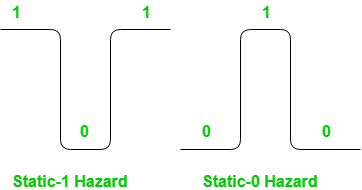
\includegraphics[scale=0.8]{./2222.png}
	%\caption{}
\end{center}

Detection of Static hazards using K-map:
Lets consider static-1 hazard first. To detect a static-1 hazard for a digital circuit following steps are used:


\begin{itemize}
	\item Step-1: Write down the output of the digital circuit, say Y.
	\item Step-2: Draw the K-map for this function Y and note all adjacent 1’s.
	\item Step-3: If there exists any pair of cells with 1’s which do not occur to be in the same group ( i.e. prime implicant), it indicates the presence of a static-1 hazard. Each such pair is a static-1 hazard.
\end{itemize}


Lets have an example:

Example – Consider the circuit shown below.



\begin{center}
	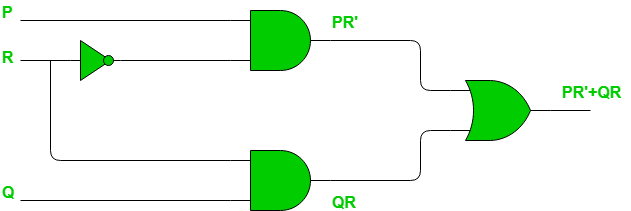
\includegraphics[scale=0.6]{./333-2.png}
	%\caption{}
\end{center}


We have output, say F, as:

$$
F(P,Q,R) = QR + PR^{\prime} = \sigma{m{3,4,6,7}}
$$

Lets draw the K-map for this Boolean function as follows:


\begin{center}
	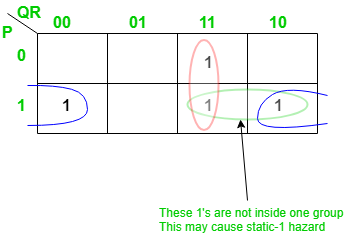
\includegraphics[scale=0.8]{./555-3.png}
	%\caption{}
\end{center}

The pair of 1’s encircled as green are not part of the grouping/pairing provided by the output of this Boolean function. This will cause a static-1 hazard in this circuit.

\section{Removal of static-1 hazard:}


Once detected, a static-1 hazard can be easily removed by introducing some more terms (logic gates) to the function (circuit). The most common idea is to add the missing group in the existing Boolean function, as adding this term would not affect the function by any mean but it will remove the hazard. Since in above example the pair of 1’s encircled with blue color causes the static-1 hazard, we just add this as a

$$
F(P,Q,R) = QR + PR^{\prime} + PQ = \sigma{m{3,4,6,7}}
$$


Note that there is no difference in number of minterms of this function. The reason is that the static-1 hazards are based on how we group 1’s (or 0’s for static-0 hazard) for a given set of 1’s in K-map. Thus it does not make any difference in number of 1’s in K-map. The circuit would look like as shown below with the change made for removal of static-1 hazard.



\begin{center}
	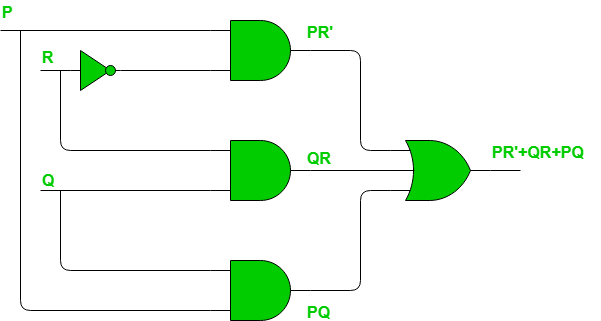
\includegraphics[scale=0.6]{./6666.png}
	%\caption{}
\end{center}


Similarly for Static-0 Hazards we need to consider 0’s instead of 1’s and if any adjacent 0’s in K-map are not grouped into same group that may cause a static-0 hazard. The method to detect and resolve the static-0 hazard is completely same as the one we followed for static-1 hazard except that instead of SOP, POS will be used as we are dealing with 0’s in this case.




\end{document}